% --------------------------------------------------------------
% This is all preamble stuff that you don't have to worry about.
% Head down to where it says "Start here"
% --------------------------------------------------------------

\documentclass[12pt]{article}

\usepackage{minted}
\usepackage{url,graphicx}
\usepackage{proof}
\usepackage{framed}
\usepackage{etaremune}

\usepackage[margin=1in]{geometry}
\usepackage{amsmath,amsthm,amssymb,amsfonts}
\usepackage{paralist}

\usepackage[most]{tcolorbox}

\definecolor{bg}{rgb}{0.9,0.9,0.9}%-- try others later
\definecolor{lightgray}{rgb}{0.95,0.95,0.95}%-- try others later
\definecolor{block-gray}{gray}{0.9}%-- try others later
\definecolor{dark-gray}{gray}{0.86} %-- try others later
\definecolor{light-gray}{gray}{0.96} %-- try others later
\newtcolorbox{myquote}{colback=block-gray,breakable,boxrule=0pt}
\newtcolorbox{mydarkquote}{colback=dark-gray,breakable,boxrule=0pt}
\newtcolorbox{mylightquote}{colback=light-gray,breakable,boxrule=0pt}


% 1. To get version suitable for students to populate,
%    remove the contents of the \ignoreSoln{..body..}
%
% 2. To get a version suitable for generating PDF 
%    without solutions, remove the #1 below
%
% 3. To generate solutions, keep the #1 below
%
% 4. Assigned grader fills \ignoreSoln{..body..}
%    and also provides his/her feedback to student
%    and policy followed for point deduction
%    So design policy before grading begins.

\newcommand{\ignoreSoln}[1]{#1}   
%\newcommand{\ignoreModel}[1]{#1} 


\newcommand{\bigset}[2]{\big\{\;#1\;:\;#2\;\big\}}
\newcommand{\N}{\mathbb{N}}
\newcommand{\Z}{\mathbb{Z}}
\newcommand{\R}{\mathbb{R}}
\newcommand{\Np}{\mathbb{N^{+}}}

\newenvironment{theorem}[2][Theorem]{\begin{trivlist}
\item[\hskip \labelsep {\bfseries #1}\hskip \labelsep {\bfseries #2.}]}{\end{trivlist}}
\newenvironment{lemma}[2][Lemma]{\begin{trivlist}
\item[\hskip \labelsep {\bfseries #1}\hskip \labelsep {\bfseries #2.}]}{\end{trivlist}}
\newenvironment{exercise}[2][Exercise]{\begin{trivlist}
\item[\hskip \labelsep {\bfseries #1}\hskip \labelsep {\bfseries #2.}]}{\end{trivlist}}
\newenvironment{reflection}[2][Reflection]{\begin{trivlist}
\item[\hskip \labelsep {\bfseries #1}\hskip \labelsep {\bfseries #2.}]}{\end{trivlist}}
\newenvironment{proposition}[2][Proposition]{\begin{trivlist}
\item[\hskip \labelsep {\bfseries #1}\hskip \labelsep {\bfseries #2.}]}{\end{trivlist}}
\newenvironment{corollary}[2][Corollary]{\begin{trivlist}
\item[\hskip \labelsep {\bfseries #1}\hskip \labelsep {\bfseries #2.}]}{\end{trivlist}}

\DeclareMathSizes{14}{14}{14}{14}

\setlength{\textwidth}{4in}

\begin{document}

% --------------------------------------------------------------
%                         Start here
% --------------------------------------------------------------

%\renewcommand{\qedsymbol}{\filledbox}


\begin{center}
\begin{large}
  CS 3100, Fall 2019, \\
  Basic Battery of Problems for Midterm-2
\end{large}
\end{center}

\date{}

%-> \item (Simple CFG patterns)
%-> \item (Designing/understanding CFG)
%-> \item (Identifying languages to be CFL or not; PL proof if not)
%-> \item (Drawing parse trees to show words to be in L(G))
%-> \item (Consistency)
%-> \item (Completeness)
%-> \item (Ambiguous grammars)
%-> \item (Disambiguation)
%-> \item (Linearity; DFA to CFG conversion)
%-> \item (CFL Pumping Lemma)
% \item (PDA basics)
% \item (Designing/understanding simple PDAs)
%-> \item (Conversion of CFG to PDA)
% \item (Ambiguity in PDAs designed out of ambiguous CFG)

\begin{large}
  
\section{Some Student FAQs}


\begin{enumerate}

\item Is dealing with strings of the form $0^M 1^N$ for $M>N$ easier in a PDA compared to a language
  where the number of $0$'s are required to be greater than the number of $1$'s? Why?

\item What are final states? What are accept states? Are they the
  same? (Answer: yes; we tend to use ``accept'' states a bit more
  with TM, because that is a final state in which the TM halts,
  and we then know that the TM has accepted the input---i.e.
  not rejected the input.)
  
\item How do you include an ``epsilon move'' in a PDA? This
  is a move akin to an NFA's epsilon move.

\item How do you feed the shortest string in these languages
  to a TM:
  \begin{compactenum}
  \item  \( \{0^i0^i\#0^i \;:\;  i\ge 0 \} \)
  \item  \( \{0^i\#0^i0^i \;:\;  i > 0 \} \)
  \item  \( \{w\#ww \;:\; w\in\{0,1\}^*\} \)
  \end{compactenum}

\item A CFL is a language for which there is a PDA that serves
  as an exact acceptor.
  That is, $L$ is a CFL, if and only if there is a PDA $P$
  such that
\begin{compactitem}
\item $w\in L \Rightarrow\;$ $P$ when run on $w$ will
  end up in a final state {\bf at which point the input is fully
    consumed.} {\em Note that unlike with a TM,} a PDA
    can continue on and transition to other states.
    But since the input is fully consumed, those transitions
    do not read additional input.
  
  \item $w\notin L \Rightarrow\;$ $M$ when run on $w$ will {\bf not}
    reach one of the final states {\bf with the input
      fully consumed.}
  \end{compactitem}

\item Can a PDA ``loop'' (i.e., infinitely loop) like a TM?
  Yes it can: one can simply sit in a tight loop and push
  things on the stack.
  %
  However, such excursions are useless. While this is
    somewhat difficult to prove in the PDA-land, it is much easier
    to prove in the CFG-land. Here is how: (1)~convert the PDA
    to a CFG (this conversion is not that hard, and found in
    many books out there). (2)~See if the CFG can parse $w$ using
    one of the standard parsing methods. This construction shows
    that we don't need to be ``stuck'' in the PDA infinite loops
    before deciding whether $w$ is accepted or not.

  \item Answer these questions either thinking of a PDA or a CFG.
    Ideally, you must provide an answer through both means.
  \begin{compactenum}
  \item Is the union of two CFLs a CFL?
  \item Is the concatenation of two CFLs a CFL?
  \item Is the Kleene-star of a CFL a CFL?
  \item Is the intersection of two CFLs a CFL?
    Hint: think of the intersection of
    \begin{compactenum}
    \item \( \{a^m b^n c^n \;:\; m,n \ge 0 \} \)
    \item \( \{a^n b^n c^m \;:\; m,n \ge 0 \} \)
    \end{compactenum}
  \item Based on your answer to the above questions,
    can the complement of a CFL be a CFL?
  \end{compactenum}
  
\item
  A recursively enumerable language is one for which
  there is a TM that serves as an exact acceptor.
  That is, $L$ is RE (recursively
  enumerable)\footnote{Not ``$L$ is a regular expression''}
  if and only if there is a TM $M$ such that
  \begin{compactitem}
  \item $w\in L \Rightarrow\;$ $M$ when run on $w$ will halt
    in one of the accept states of $M$
  \item $w\notin L \Rightarrow\;$ $M$ when run on $w$ will {\bf not}
    halt
    in one of the accept states of $M$. (This may mean that
    $M$ may halt in a non-accept state (this is compactly
    stated as
    ``M rejects'') or $M$ may loop (we can't tell this; so
    long ans $M$ does not accept, it is the other two possibilities,
    namely rejection or looping, that must be true)
  \end{compactitem}
  %
  \item Answer these questions either thinking of a PDA or a CFG.
    Ideally, you must provide an answer through both means.
  \begin{compactenum}
  \item Is the union of two RE languages RE?
  \item Is the concatenation of two RE languages RE?
  \item Is the Kleene-star of an RE language RE?
  \item Is the complement of an RE language RE?
  \item Is the intersection of two RE languages RE?
  \end{compactenum}

\item What are the two rules that help translate {\bf any} CFG into a PDA?
  
\item This CFG arose naturally in one of my adventures:
\begin{verbatim}
S -> ( W S | ''
W -> ( W W | )
\end{verbatim}
\begin{compactitem}
\item What familiar language is this CFG describing?
\item How do you show it is consistent?
  (Exam questions won't be this hard, but this is given for your own curiosity.)
\item How do you show it is complete?
  (Exam questions won't be this hard, but this is given for your own curiosity.)  
\end{compactitem}

\item What are two classes of strings in the {\bf complement} of the language $ww$ (set of strings of the
  form $w$ followed by $w$; examples being $01001 \; 01001$)?
  How do you write a CFG for the complement of the $ww$ language?

\item Suppose there is a CFG production for nonterminal $A$. How do you write a CFG production
  for the language $A^*$?

\item Suppose there is a CFG production for nonterminals $A$ and $B$. How do you write a CFG production
  for the language $(A+B)$?

\item How do you go about designing a CFG for the set of strings where the \#1's exceeds the \#0's (Assignment 4 question)?
\item[] Hint: don't try to do it in one rule! It won't work. Try to conquer the ``equality'' and ``ascending'' parts
  separately. Then stitch together using the tricks mentioned in the earlier questions. You'll end up with many CFG
  rules (4 or 5 in my estimate).

\item Design a PDA for the set of strings with twice as many $b$'s as $a$'s.
\item[] Hint: You have to maintain a discipline wrt the things on the stack. I'll also show you how to interactively arrive
  at the PDA design, executing piece by piece.

\end{enumerate}

\section{Battery of Questions}


\begin{enumerate}
  
\item (Simple CFG patterns)
Write a CFG for $0^*$


\item (Simple CFG patterns)
  Write a CFG for $10^*1$


\item (Simple CFG patterns)
  Write a CFG for the set of odd-length palindromes over $\{0,1\}$


\item (Simple CFG patterns)
  Write a CFG for the set of odd-length strings over $\{0,1\}$


\item (Simple CFG patterns)
  Write a CFG for the language $0(00)^*$


\item (Simple CFG patterns)
  How many productions will there be in a CFG for the language over $\{a,b\}$
  with two $a$'s for every three $b$'s?


\item (Designing/understanding CFG)
  Given this CFG with {\tt S} as the start symbol,
\begin{verbatim}
S -> XSX | R
R -> aTb | bTa
T -> XTX | X | ''
X -> a|b
\end{verbatim}
  answer the following questions:
\begin{compactenum}
\item What are the terminals and nonterminals?

\item How many productions are there (the \verb\|\ is an abbreviation; de-abbreviate those and count)
  
\item Draw a parse tree for {\tt abaa}
  
\item Draw a parse tree for {\tt abaaa}
  
\item Write a regular expression for the language of this grammar (in general, this is impossible,
  but here you can). Please try!

    
\end{compactenum}

\item There was another ``trickster'' that I ran into for which I think
  I have a solution---will try later. Here is that one, which is
  {\bf Sipser's Problem 2.25}.
Suppose we are given a CFG $G$

\begin{verbatim}
S -> a S b | b Y | Y a
Y -> b Y | a Y | ''
\end{verbatim}

\begin{enumerate}
\item If $L(G)$ is regular, simplify it down to a regular expression.
\item If $L(G)$ is not regular, obtain a Pumping Lemma proof for that fact.
\end{enumerate}
{\bf CAN YOU??} I think I got a simplification for it.
  You are invited to try!!


\item (Designing/understanding CFG)  Design a CFG for the set of
  strings $w$ that contain at least three $1$'s ($\Sigma=\{0,1\}$)

\item (Designing/understanding CFG) Design a CFG for the  set of
  strings $w$ that are odd in length and the middle symbol is a $0$ ($\Sigma=\{0,1\}$).
  Draw a parse tree for $01011$ using this grammar.

\item \label{paren-qn} (Designing/understanding CFG) Design a CFG for the  set of
  balanced parentheses, square brackets, and braces. For example,
  here are the legal strings in this language:
  \begin{compactenum}
  \item   \verb| ()[]{} |
  \item   \verb|  {{[()()][{}]}} |
  \item   \verb| [ {{[()()][{}]}} ] |
  \item   \verb| [ {{[()()][{}]}} {[()()][{}]} ] ()[]{} |    
  \end{compactenum}

\item Argue the consistency and completeness of the grammar you arrive at in Question~\ref{paren-qn}.
  To simplify the case analysis during completeness,
  ignore \verb|{| and \verb|}| (i.e. assume the strings only consist of
  \verb|(|, \verb|)|, \verb|[|, or \verb|]| -- of course, well-parenthesized).

\item (Designing/understanding CFG)
  Write a CFG for the set of strings over $\{a,b,c\}$ where the number of $a$s
  equals the number of $b$s plus the number of $c$s.


\item \label{iEQjORjEQk}
  (Designing/understanding CFG) Design a CFG for the language of strings
  \( \{a^i b^j c^k \;:\; i=j\; {\rm or}\; j=k \} \)

\item \label{iEQjORiEQk}
  (Designing/understanding CFG) Design a CFG for the language of strings
  \( \{a^i b^j c^k \;:\; i=j\; {\rm or}\; i=k \} \)
  
\item (Designing/understanding CFG) Design a CFG for the language of strings
  of the form $(w a w^R)(w b w^R)$ where $w\in\{0,1\}^*$ and $a,b\in\{0,1\}$, with
  $a\neq b$.


\item (Designing/understanding CFG)
  Consider the expression grammar
\begin{verbatim}
  E -> E + E | E * E | E ** E | 2 | (E)
\end{verbatim}
Here, \verb|**| stands for exponentiation. 
\begin{compactenum}
\item Define grammar ambiguity.
\item Is this grammar ambiguous? Why? (Present through a clear example.)
\item Disambiguate this grammar. While disambiguating,
  assign exponentiation the highest precedence, followed
  by \verb|*| (multiplication), and finally addition (\verb|+|).
  
\item Provide an informal proof that the grammar has been disambiguated.
\end{compactenum}


\item (Designing/understanding CFG)
  Consider the regular expression grammar for regular expressions over $\Sigma=\{a\}$, with
  \verb|@| used to represent Epsilon (for convenience).
\begin{verbatim}
  E -> E E | E* | E+E | @ | a
\end{verbatim}
%--
\begin{compactenum}
\item Define grammar ambiguity.
\item Is this grammar ambiguous? Why? (Present through a clear example.)
\item Disambiguate this grammar.
  While disambiguating, we want regular expression concatenation to have higher precedence than regular
  expression union (\verb|+|), and Kleene star (\verb|E*|) to have higher precedence
  than concatenation.

\item Provide an informal proof that the grammar has been disambiguated.
\end{compactenum}

\item Argue that the syntax of regular expressions is context-sensitive
  while the syntax of CFG productions is regular.


\item (Conversion of CFG to PDA)  {\bf Convert each and every CFG you designed
  earlier into a PDA.} Argue why this PDA works.

\item (Identifying languages to be CFL or not; PL proof if not)
  Is the language $0^n 1^n$ for $n\ge 0$ a CFL? If so, present a CFG and a PDA for it.
  If not, provide a PL proof for it. ({\bf HINT:} See if you can design
  a PDA for the language; if it appears impossible, it is likely a CFL.)
  
\item (Identifying languages to be CFL or not; PL proof if not)
  Is the language $0^n 1^n 0^m 1^m$ for $m,n\ge 0$ a CFL? If so, present a CFG and a PDA for it.
  If not, provide a PL proof for it.

\item (Identifying languages to be CFL or not; PL proof if not)
  Is the language $0^n 1^n 0^m 1^m$ for $m,n\ge 0$ and $m=n$ a CFL? If so, present a CFG and a PDA for it.
  If not, provide a PL proof for it.  

\item (Identifying languages to be CFL or not; PL proof if not)
  Is the language $0^n 1^n 0^m 1^m$ for $m,n\ge 0$ and $m\ge n$ a CFL? If so, present a CFG and a PDA for it.
  If not, provide a PL proof for it.  
  
\item (Identifying languages to be CFL or not; PL proof if not)
  Is the language $0^n 1^n 0^m 1^m$ for $m,n\ge 0$ and $m>n$ a CFL? If so, present a CFG and a PDA for it.
  If not, provide a PL proof for it.

\item (From Sipser)(Identifying languages to be CFL or not; PL proof if not)
  This is the language:
  \( \{a^i b^j c^k \;:\; i\leq j\leq k,\; i,j,k\ge 0\} \)

\item (From Sipser)(Identifying languages to be CFL or not; PL proof if not)
  This is the language, where \verb|#| is a separator:
  \( \{0^n\# 0^{2n} \# 0^{3n} \;:\; n\ge 0\}\)

\item (From Sipser)(Identifying languages to be CFL or not; PL proof if not)
  This is the language, where \verb|#| is a separator:
  \( \{w\# x \;:\; w\; \rm{is} \; \rm{a}\; \rm{subtring}\; \rm{of}\; x\}\) where $w,x\in\{a,b\}^*$.
  $w$ is a substring of $x$ if $w$ is a contiguous sequence of characters present in $x$.

\item (Designing/understanding CFG) What is the language
  generated by this CFG? Design a PDA for it both using direct design (without
  converting a CFG to a PDA)
  and through conversion. Here, \verb|!| is simply a separator.
\begin{verbatim}
  T -> 0T | T0 | !
\end{verbatim}

\item \label{lin-qn}
  (Designing/understanding CFG) Consider this CFG once again:
\begin{verbatim}
  T -> 0T | 1T | !
\end{verbatim}
\begin{compactenum}
\item Is this CFG purely left-linear?
\item Is it purely right-linear?
\item Is its language regular?
\item What is the theorem pertaining to mixed linear CFG productions
  and whether the language is regular or not? State it clearly
  as an implication or a bi-implication. Does this theorem help you judge
  whether this language is regular or not?
\end{compactenum}

\item (Designing/understanding CFG)
  Reverse this CFG. 
\begin{verbatim}
  T -> 0T | 1T | !
\end{verbatim}
Call the new nonterminal {\tt Tr} for ``T reversed.''
Then answer Question~\ref{lin-qn}.


\item (Linearity; DFA to CFG conversion)
  Convert this DFA to a CFG by the direct approach of converting
  transitions to CFG productions.
  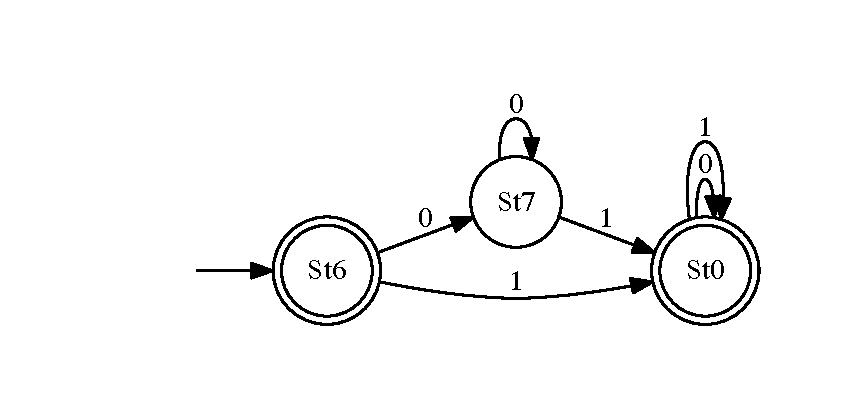
\includegraphics[width=.4\linewidth]{DO_odd1s.pdf}

  
\item (Linearity; DFA to CFG conversion)
  Consider this CFG once again:
\begin{verbatim}
  T -> 0T | T0 | !
\end{verbatim}
\begin{compactenum}
\item Is this CFG purely left-linear?
\item Is it purely right-linear?
\item Is its language regular?
\item What is the theorem pertaining to mixed linear CFG productions
  and whether the language is regular or not? State it clearly
  as an implication or a bi-implication.
\end{compactenum}

  
\item (Designing/understanding CFG) What is the language
  generated by this CFG? Design a PDA for it both using direct design (without
  converting a CFG to a PDA)
  and through conversion. Here, \verb|!| is simply a separator.
\begin{verbatim}
  S -> 0S00 | !
\end{verbatim}

  
\item (PDA basics)
  In a few sentences describe the language of the PDA presented below
  (Jove commands to generate the PDA are also shown, for added information).
  
  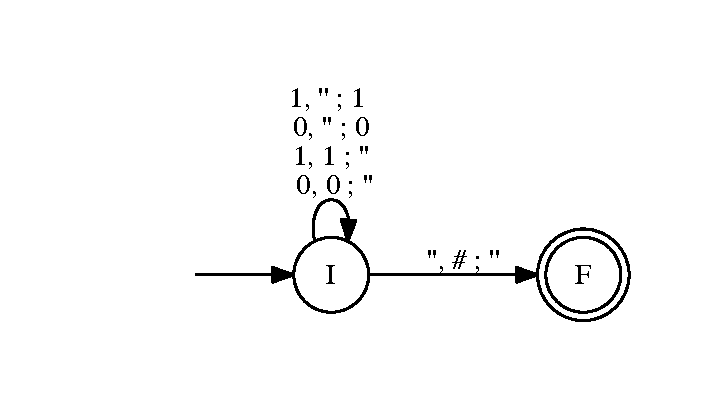
\includegraphics[width=.4\linewidth]{DO_pda1.pdf}

  Why is this
  PDA's language not that of the set of palindromes over $\{0,1\}$?
%---
\begin{minted}
[
 frame=lines
,framesep=2mm
,baselinestretch=1.2
,bgcolor=bg
,fontsize=\small
%linenos
]
{python}
pda1 = md2mc('''PDA
I : 0,''; 0 | 1,''; 1 | 0,0; '' | 1,1; '' -> I
I : '', #; '' -> F
''')
DO_pda1 = dotObj_pda(pda1, FuseEdges="True")
DO_pda1.render()
DO_pda1
\end{minted}
%---



\item (PDA basics)
  In a few sentences describe the language of the PDA presented below. 
  
  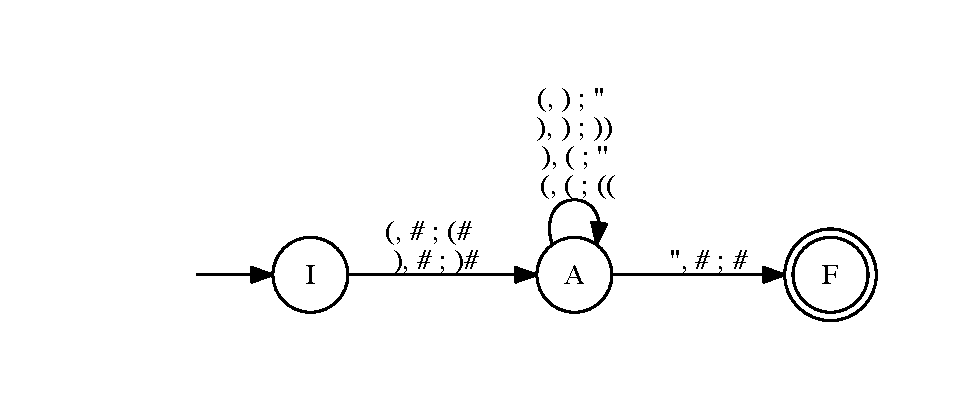
\includegraphics[width=.4\linewidth]{DO_pda2.pdf}
  
  Why is this
  PDA's language not that of the Dyck language (which is the set of perfectly
  nested parentheses, such as {\tt ()()} or {\tt (())} or {\tt ((())())}.
  %
  What changes will you make to this PDA's design to convert it into
  a PDA for the Dyck language?
%---
\begin{minted}
[
 frame=lines
,framesep=2mm
,baselinestretch=1.2
,bgcolor=bg
,fontsize=\small
%linenos
]
{python}
pda2 = md2mc('''PDA
I : (,#; (# | ),#; )# -> A
A : (,(; (( | ),); )) | (,); '' | ),(; '' -> A
A : '',#; # -> F
''')
DO_pda2 = dotObj_pda(pda2, FuseEdges="True")
DO_pda2.render('DO_pda2')
DO_pda2
\end{minted}
%---

\item (Designing/understanding simple PDA)
  Directly design a PDA (without converting from a CFG) for the language of
  Question~\ref{paren-qn}.

\item   (Designing/understanding simple PDA)
  Suppose $x,w\in\{a,b\}^*$ and $x$ is a substring of $w^R$. An exmaple
  would be $x=ab$ and $w=bbab$ whereupon $w^R=babb$ and you see that $x$ is a substring of $w^R$.
  In any case, $x$ is a substring of $w$-reversed.
  Directly design a PDA for the language\\
  $\{x\!w^R\}$ under these conditions, where \verb|!| is a separator.

\item (Designing/understanding simple PDA)
  Directly design a PDA for the language of Question~\ref{iEQjORjEQk}.


\item (Designing/understanding simple PDA)
  Directly design a PDA for the language of Question~\ref{iEQjORiEQk}.

\item (Designing/understanding simple PDA)
  Directly design a PDA for the language of strings over $\{0,1\}$ where the
  number of $1$'s is strictly more than the number of $0$'s.


\item (Designing/understanding simple PDA)
  Directly design a PDA for the language of strings $w$ over $\{a,b\}$ such
  that $w$ has twice as many $b$'s as there are $a$'s.

\item Design a CFG and PDA for these languages. If they are not CFL,
  then write a PL proof:

  \begin{compactenum}
  \item \(L_1 =  \{a^i b^j c^k d^l \;:\;
    \textrm{if}\; i=2\; \textrm{then} \; j=k \textrm{else} \; k=l \)
  \item \(reverse(L_1)\)
  \end{compactenum}

\item (From Chapter 11)
  Argue that this language is
a CFL by building a
CFG for it. Answer for both 
cases of `OP' listed below:
\[ L_{abcd} = \{ a^i b^j c^k d^l \;:\;   
                          i,j,k,l\ge 0 \; 
 {\rm and} \;
 ((i=j) \;
 {\rm OP}\;
 (k=l))
 \} \]
 \begin{compactenum}
   \item (Case 1) OP is $AND$
   \item (Case 2) OP is $OR$
 \end{compactenum}

\item (From Chapter 11)
 Show that $L_{acbd}$ is not context-free if $OP$ is
  $AND$ but is context-free if $OP$ is $OR$:
 
\[ L_{acbd} = \{ a^i c^k b^j d^l \;:\;   
                          i,j,k,l\ge 0 \; 
 {\rm and} \;
 ((i=j) \;
  OP\;
 (k=l))
 \} \]


\item (Simple TM question)
  Read the description of this simple TM

  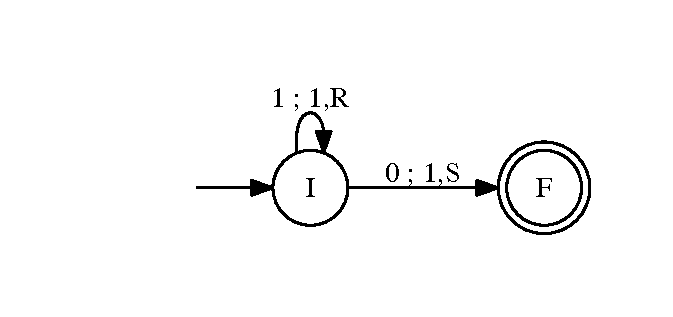
\includegraphics[width=.6\linewidth]{TM0to1.pdf}  

  Now answer these questions:
  \begin{compactenum}
  \item What does this TM do upon input \verb|101|?
  \item What does this TM do upon input \verb|111|?
  \item What is the language of this TM? 
  \end{compactenum}


\item (Simple TM question)
  Read the description of this simple TM

  \hspace{-1cm} 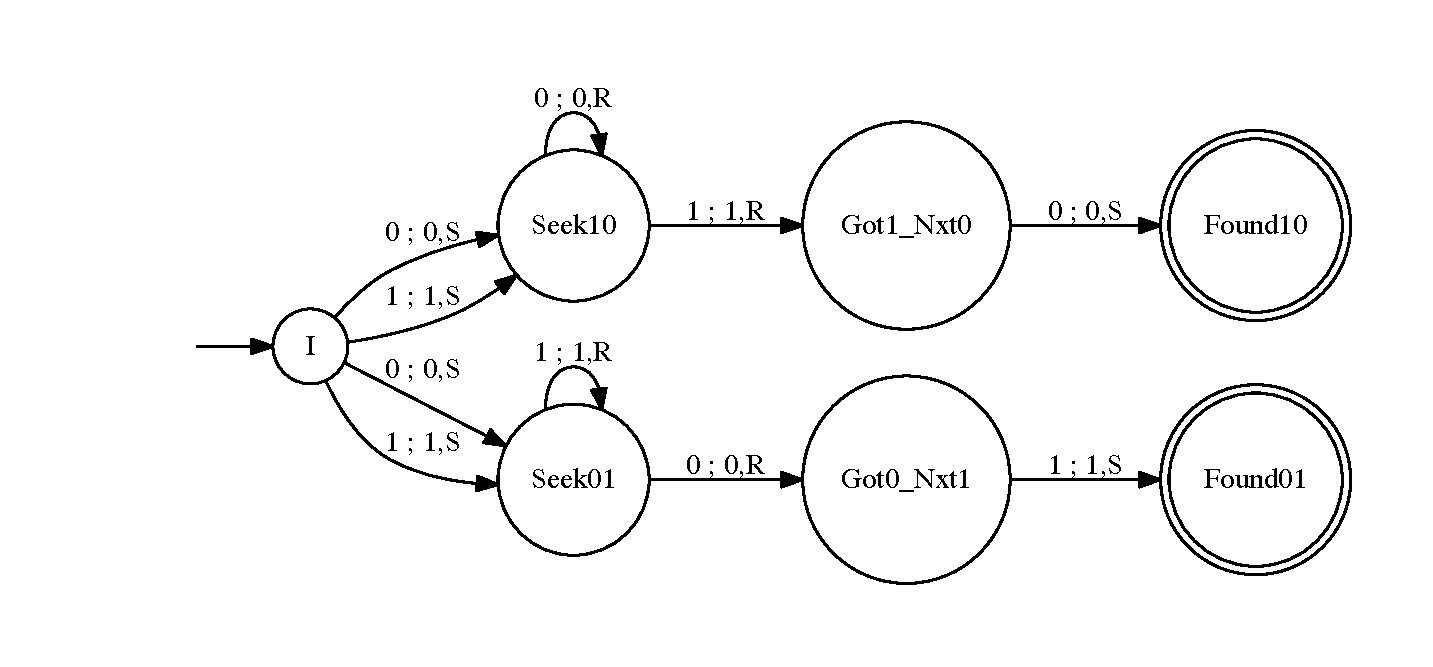
\includegraphics[width=.9\linewidth]{TM01OR10.pdf}  

  Now answer these questions:
  \begin{compactenum}
  \item What does this TM do upon input \verb|1111|?
  \item What does this TM do upon input \verb|0010|?
  \item What is the language of this TM? 
  \end{compactenum}
  
 
\end{enumerate}


\end{large}

\end{document}
%==
